\section{Auswertung}

Alle Ausgleichsrechnungen werden mit dem Paket \texttt{scipy.optimize.curve\_fit}  aus \texttt{Python 3.7.3} durchgeführt.
Die Unsicherheit auf die gemessenen Ereignisse $N$ beträgt $\sigma_\text{N} = \sqrt{N}\,$.
Für Rechnungen mit fehlerbehafteten Größen wird das Paket \texttt{uncertainties} aus \texttt{Python 3.7.3} verwendet.

\subsection{Kanal Kalibration}

Anhand der \ce{^{152}Eu}-Quelle sollen die Kanäle des Germaniumdetektors auf die Energien kalibriert werden.
Die Emissionsenergien von \ce{^{152}Eu} und die dazugehörigen Emissionswahrscheinlichkeiten sind bekannt und in Tabelle \ref{tab:Eu_Emisionsenergie} aufgelistet \cite{Eu_Emision}.
Aus dem aufgenommenen Spektrum von \ce{^{152}Eu} lassen sich die Kanäle der Photopeaks bestimmen.
Es werden die relativen Abstände der Kanalnummern der Photopeaks und der Emissionsenergien aus Tabelle \ref{tab:Eu_Emisionsenergie} gebildet und übereinander gelegt.
Mit den übereinander liegenden Punkten lassen sich die Emissionsenergien den Kanalnummern zuordnen.
Die Übereinstimmung der relativen Abstände ist dabei so genau, dass auf eine Bestimmung der Unsicherheiten verzichtet wird.

Um jedem Kanal eine Energie zuzuweisen, wird eine lineare Ausgleichsrechnung der Form $E(K) = m*K+b$ durchgeführt.
Diese ist in Abbildung \ref{fig:Channel_Kalibration} dargestellt.
Anhand der Parameter $m$ und $b$ kann jedem Kanal eine Energie

\begin{equation}
  E(K) = (0.21 \pm \num{3e-5})\,\si{\kilo\electronvolt} \cdot K + \SI{1.33(14)}{\kilo\electronvolt}
  \label{channel_kal}
\end{equation}
zugeordnet werden.
Aufgrund der kleinen Unsicherheiten der Parameter $m$ und $b$ werden jene in folgenden Rechnungen vernachlässigt.

\begin{figure}[H]
  \centering
  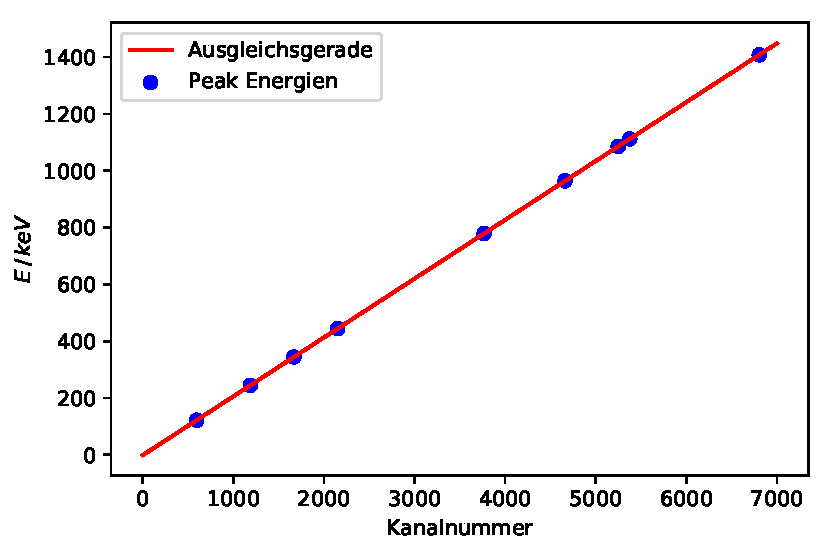
\includegraphics[width = .7\textwidth]{../Plots/Channel_Kalibration.pdf}
  \caption{Ausgleichsrechnung zur Energiekalibration der Kanalnummern.}
  \label{fig:Channel_Kalibration}
\end{figure}

\subsection{Vollenergienachweiswahrscheinlichkeit}

Zur Bestimmung der Vollenergienachweiswahrscheinlichkeit $Q$ muss zuerst die Aktivität der \ce{^{152}Eu}-Quelle berechnet werden.
Der Anleitung zufolge hatte die Quelle am 01.10.2000 eine Aktivität von $A_\text{0} = (4130 \pm 60)\,\si{\becquerel}$.
Mit einer Halbwertszeit von 13 Jahren und 196 Tagen hat die Quelle zum Tag der Messung eine Aktivität von
\begin{equation*}
  A(04.11.2019) = (1552 \pm 23)\,\si{\becquerel}\,.
\end{equation*}
%Mit der Unsicherheit
%\begin{equation*}
%  \sigma_A = \exp{\left(-\ln{(2)} \frac{t}{T_{\sfrac{1}{2}}}\right)} \cdot \sigma_{A_0} \, .
%\end{equation*}

Die Quelle ist $\SI{6}{\centi\meter}$ von dem Detektor entfernt angebracht. Mit einem Abstand von $\SI{1.5}{\centi\meter}$ zwischen Detektormantel und Detektor ergibt sich ein Gesamtabstand von $h = \SI{7.5}{\centi\meter}$ zwischen Quelle und Detektorfläche.
Die Detektorfläche hat einen Durchmesser von $d = \SI{45}{mm}$.
Für den Raumwinkel $\Theta$ folgt nach Gleichung \eqref{eqn:Raumwinkel}
\begin{equation*}
   \Theta = \num{1.04} \, .
\end{equation*}

Für die Photopeaks der \ce{^{152}Eu} Quelle werden die Peakinhalte $N_\text{P,\ce{Eu}}$ bestimmt, welche in Tabelle \ref{tab:Eu_Emisionsenergie} aufgelistet sind.
Zur Bestimmung der Peakinhalte werden die Ereignisse in einem Bereich von \SI{\pm2.5}{\kilo\electronvolt} um das Maximum aufsummiert. Die Wahl dieser Breite lässt sich in Kapitel \ref{sec:Cs} nachvollziehen.

Die Vollenergienachweiswahrscheinlichkeit des Detektors kann somit für die Energien der Photopeaks nach Gleichung \eqref{eqn:Vollenergienachweiswahrscheinlichkeit} bestimmt und in Tabelle \ref{tab:Eu_Emisionsenergie} eingetragen werden.

Die Vollenergienachweiswahrscheinlichkeiten werden in Abbildung \ref{fig:Vollenergienachweiswahrscheinlichekeit} gegen die Emissionsenergien aufgetragen und es wird eine Ausgleichsrechnung mit einer Potenzfunktion der Form
\begin{equation}
  Q(E) = a \cdot E^b
  \label{eqn:Eff}
\end{equation}
durchgeführt.
Für die Parameter $a$ und $b$ ergibt sich
\begin{align*}
   a &=  \SI{6.9(27)}{}\, ,\\
   b &=  \SI{-0.85(7)}{}\, .\\
\end{align*}

\begin{figure}[H]
   \centering
   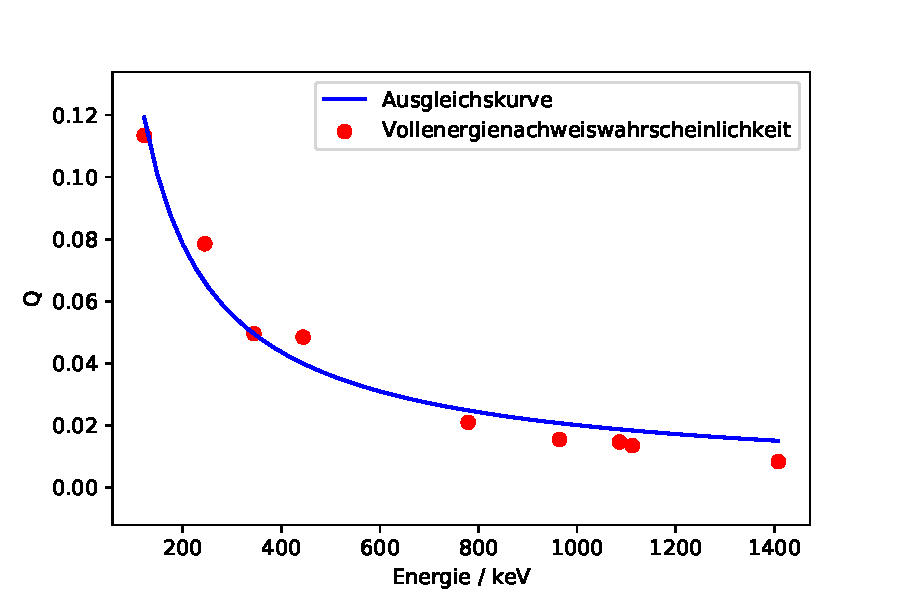
\includegraphics[width = .7\textwidth]{../Plots/Effizienz.pdf}
   \caption{Vollenergienachweiswahrscheinlichkeit $Q$ des Detektors als Funktion der Photonenenergie.}
   \label{fig:Vollenergienachweiswahrscheinlichekeit}
\end{figure}

\begin{figure}[H]
  \centering
  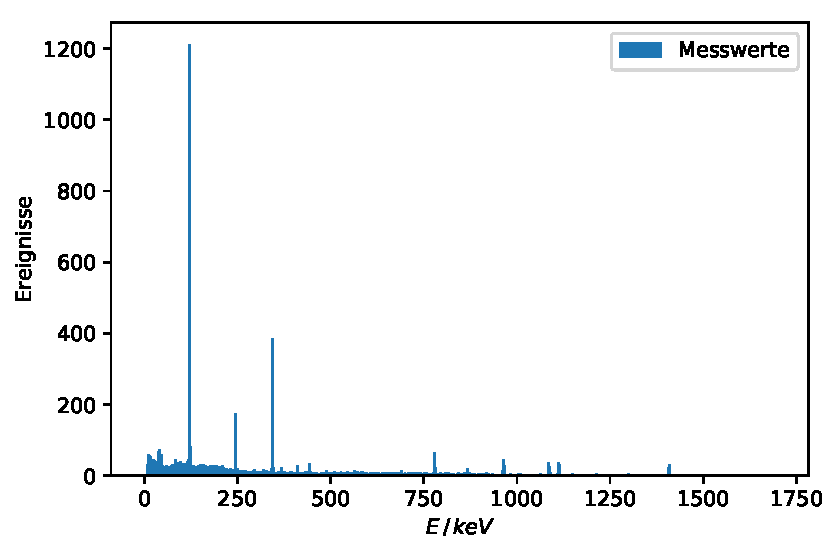
\includegraphics[width=.7\textwidth]{../Plots/Eu_Spektrum.pdf}
  \caption{Spektrum der \ce{^152Eu} Quelle.}
  \label{fig:Eu_Spektrum}
\end{figure}

\begin{table}[H]
   \centering
   \caption{Emissionsenergien und zugehörige Emissionswahrscheinlichkeiten von \ce{^{152}Eu} sowie Peakinhalte und Vollenergienachweiswahrscheinlichkeit.}
   \label{tab:Eu_Emisionsenergie}
   \begin{tabular}{cccc}
     \toprule
     $E_\text{Emission} \, / \, \si{\kilo\electronvolt}$  \cite{Eu_Emision} & $W_\text{Emission} \, / \,  \si{\percent}$  \cite{Eu_Emision} & $N_\text{P,\ce{Eu}}$ & $Q$ \\
     \midrule
     \num{121.78}	 & \num{28.6}	 &  \num{7.69(9)e3} & \num{0.113(2)}   \\
     \num{244.70}	 & \num{7.60}	 &  \num{1.42(4)e3} & \num{0.079(2)}   \\
     \num{344.30}	 & \num{26.50} &	\num{3.11(6)e3} &  \num{0.050(1)}   \\
     \num{443.96}	 & \num{3.01}	 &  \num{346(19)} 	 & \num{0.049(3)}  \\
     \num{778.90}	 & \num{12.90} &	\num{643(25)} 	 &  \num{0.021(1)}  \\
     \num{964.08}	 & \num{14.60} &	\num{536(23)} 	 &  \num{0.016(1)}  \\
     \num{1085.90} & \num{10.20} &	\num{355(19)} 	 &  \num{0.015(1)}  \\
     \num{1112.10} & \num{13.60} &	\num{435(21)} 	 &  \num{0.014(1)}  \\
     \num{1408.00} & \num{21.00} &	\num{417(20)} 	 &  \num{0.0084(4)}\\
     \bottomrule
 \end{tabular}
\end{table}


\subsection{Untersuchung der \ce{^137Cs}-Quelle}\label{sec:Cs}

Aus dem aufgenommenen Spektrum der \ce{^137Cs}-Quelle sollen der Photopeak und das Compton-Kontinuum näher untersucht werden.
In Abbildung \ref{fig:Cs_Photo} ist der Bereich des Photopeaks vergrößert dargestellt.
Zur Untersuchung des Peaks wird eine Ausgleichsrechnung mit einer Gauskurve der Form

\begin{equation*}
  f(x) = \frac{a}{\sqrt{2 \pi \sigma^2}} \exp{\left(\frac{-(E-E_0)^2}{2\sigma^2}\right)}
\end{equation*}

mit den Parametern

\begin{align*}
  a &= \SI{767(7)}{} \, , \\
  E_0 &= \SI{661.75(1)}{\kilo\electronvolt} \, , \\
  \sigma &= \SI{0.92(1)}{\kilo\electronvolt} \, ,
\end{align*}

für diesen Bereich durchgeführt.

Für die Halbwertsbreite $FWHM$ und die Zehntelwertsbreite $FWTM$, sowie den Peakinhalt $N_\text{P,\ce{Cs}}$ , welcher durch Summation der im Peak enthaltenen Ereignisse berechnet wird, folgt

\begin{align*}
  FWHM &= 2 \sqrt{2 \ln(2)} \cdot \sigma= \SI{2.16(2)}{\kilo\electronvolt} \, , \\
  FWTM &= 2 \sqrt{2 \ln(10)} \cdot \sigma= \SI{3.93(4)}{\kilo\electronvolt} \, , \\
  N_\text{P,\ce{Cs}} &= \SI{8.61(9)e3}{} \, .
\end{align*}

\begin{figure}[H]
  \centering
  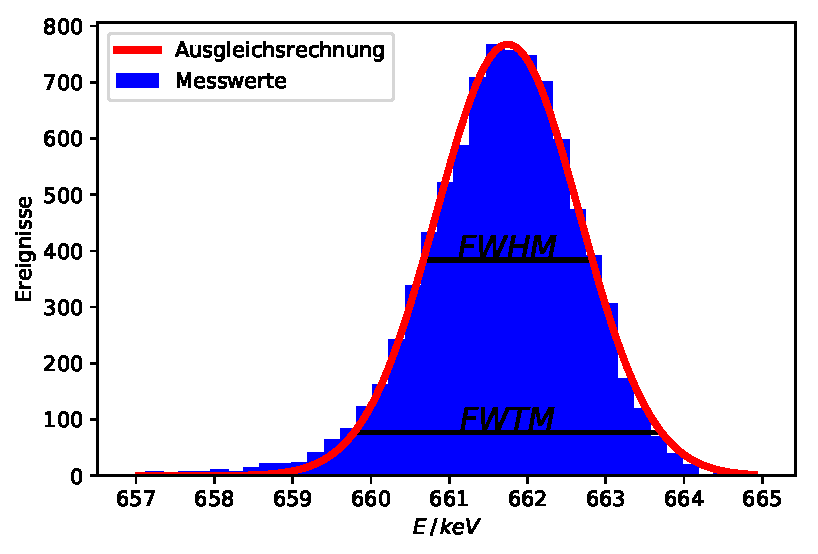
\includegraphics[width = .7\textwidth]{../Plots/Cs_Photopeak.pdf}
  \caption{Photopeak der \ce{^137Cs} Quelle mit Ausgleichsrechnung. Dargestellt sind die Halbwertsbreite und die Zentelwertsbreite.}
  \label{fig:Cs_Photo}
\end{figure}

Weiterhin wird das Compton-Kontinuum analysiert, aus diesem werden grob die Energie des Rückstreupeak $E_\text{R}$ und der Comptonkante $E_\text{C}$ abgeschätzt. Aus Gleichung \eqref{eqn:Comptonkante} und \eqref{eqn:Compton_Rückstreupeak} können,
anhand des Literaturwerts der Gamma-Emissionsenergie von $\SI{661.66}{\kilo\electronvolt}$ \cite{Cs_Emissionsenergie},
theoretische Werte für die Energien von Rückstreupeak und Comptonkante berechnet werden.
Die Ergebnisse sind in Tabelle \ref{tab:Cs_Comptonkontinuum} aufgelistet.

\begin{table}[H]
  \centering
  \caption{Photopeak, Rückstreupeak und Comptonkante von \ce{^137Cs}.}
  \label{tab:Cs_Comptonkontinuum}
  \begin{tabular}{cccc}
    \toprule
    & experimentell & theoretisch & Abweichung / $\si{\percent}$ \\
    \midrule
    $E_\text{Photo} \, / \, \si{\kilo\electronvolt}$ & \SI{661.75(1)}{} & \num{661.66} & \num{0.01} \\
    $E_\text{R} \,/\, \si{\kilo\electronvolt}$ &  $\SI{190(5)}{}$ & $\SI{184}{}$ & \num{3.3} \\
    $E_\text{C} \,/\, \si{\kilo\electronvolt}$ &  $\SI{470(5)}{}$ & $\SI{477}{}$ & \num{1.5} \\
    \bottomrule
  \end{tabular}
\end{table}

Aus der Detektorlänge $l= \SI{3.9}{\centi\meter}$ und den Extinktionskoeffizienten $\mu_\text{Photo}$ und $\mu_\text{Com.}$ kann die Extinktionswahrscheinlichkeit der \ce{^137Cs}-Quanten für den Photoeffekt und den Compton-Effekt bestimmt werden.
Dazu wird nach
\begin{equation*}
  W(E) = 1 - e^{-\mu(E) \cdot l}
\end{equation*}
die Extinktionswahrscheinlichkeit berechnet.
Die Extinktionskoeffizienten von Germanium im hier vorliegenden Energiebereich der Comptonstreuung und der Photoabsorption lauten nach \cite{nist}
\begin{align*}
  \mu_\text{Photo} = \SI{0.01}{\per\centi\meter} \, , \\
  \mu_\text{Com.} = \SI{0.36}{\per\centi\meter} \, .
\end{align*}

Die Extinktionswahrscheinlichkeit liegen somit bei
\begin{align*}
  W_\text{Photo} &= \SI{3.8}{\percent} \, , \\
  W_\text{Com.} &= \SI{75}{\percent} \, .
\end{align*}

Die Gesamtzahl an Ereignissen im Compton-Kontinuum ist mit \num{3.14(2)e4} allerdings nur um den Faktor \num{3.6} höher, als die des Photopeaks mit \num{8.61(9)e3}, während die Extinktionswahrscheinlichkeit für die Comptonstreuung um den Faktor 20 höher ist, als die der Photoabsorption.
Es lässt sich also vermuten, dass ein großer Teil der im Photopeak gemessenen Ereignisse durch mehrfache Comptonstreuung hervorgerufen wird.

\begin{figure}[H]
  \centering
  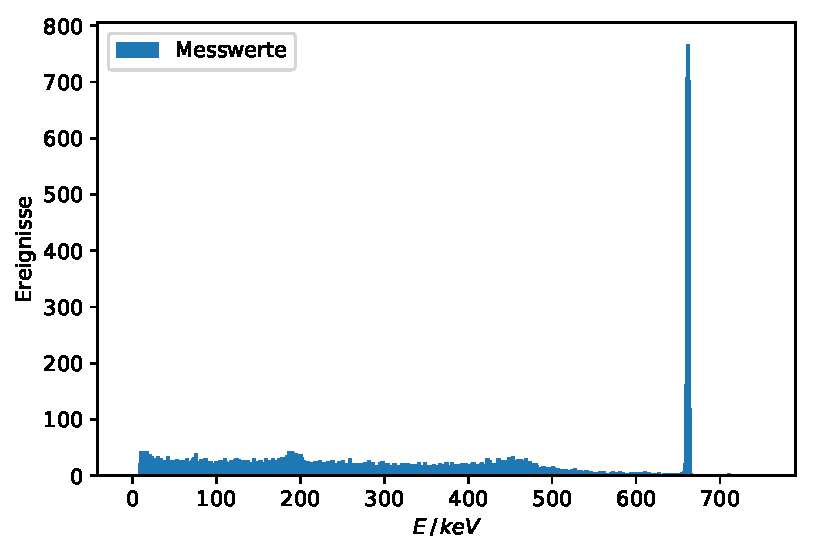
\includegraphics[width=.7\textwidth]{../Plots/Cs_Spektrum.pdf}
  \caption{Spektrum der \ce{^137Cs} Quelle.}
  \label{fig:Cs_Spektrum}
\end{figure}


\subsection{Aktivitätenbestimmung der \ce{^133Ba}-Quelle} \label{sec:Ba}

Die Aktivität der \ce{^133Ba}-Quelle am Tag der Messung kann über den Linieninhalt der Photopeaks bestimmt werden.
Um den Inhalt der Photopeaks $N_\text{P}$ zu berechnen, wird angenommen, dass die Breite der Peaks in etwa die Selbe ist, wie die Breite des \ce{^137Cs}-Photopeaks.
Somit werden die Ereignisse in einem Breich von \SI{\pm2.5}{\kilo\electronvolt} um das Maximum des Peaks aufsummiert, um den kompletten Peakinhalt zu bestimmen.
Um die Anzahl der tatsächlich in den Detektor gelangten Gammaquanten zu bestimmen, wird der Peakinhalt durch die Vollenergienachweiswahrscheinlichkeit der dazugehörigen Emissionsenergie geteilt.
Die Aktivität der \ce{^133Ba}-Quelle ergibt sich über die Summe aller Photopeaks mit der gesamten Messdauer $T_\text{M}$ und dem Raumwinkel $\Theta$ zu
\begin{equation}
  A_\text{\ce{^133Ba}}(04.11.2019) = \sum_{P} \frac{N_\text{P}}{Q_\text{P} T_\text{M} \sfrac{\Theta}{4\pi}} = \SI{1.3(7)e3}{\becquerel}
  \label{eqn:Act_Ba}
\end{equation}

Die gemessene Aktivität der \ce{^133Ba}-Quelle kann mit der errechneten Aktivität nach dem Zerfallsgesetz verglichen werden.
Die Halbwertszeit von \ce{^133Ba} beträgt 10 Jahre und 188 Tage. Mit der, auf der Probe aufgeschriebenen, Aktivität von  $A_0(1.10.2000) \approx \SI{4000}{\becquerel}$ folgt somit
\begin{equation*}
  A_\text{\ce{^133Ba,theo.}}(04.11.2019) = \SI{1335}{\becquerel} \, .
\end{equation*}

\begin{figure}[H]
  \centering
  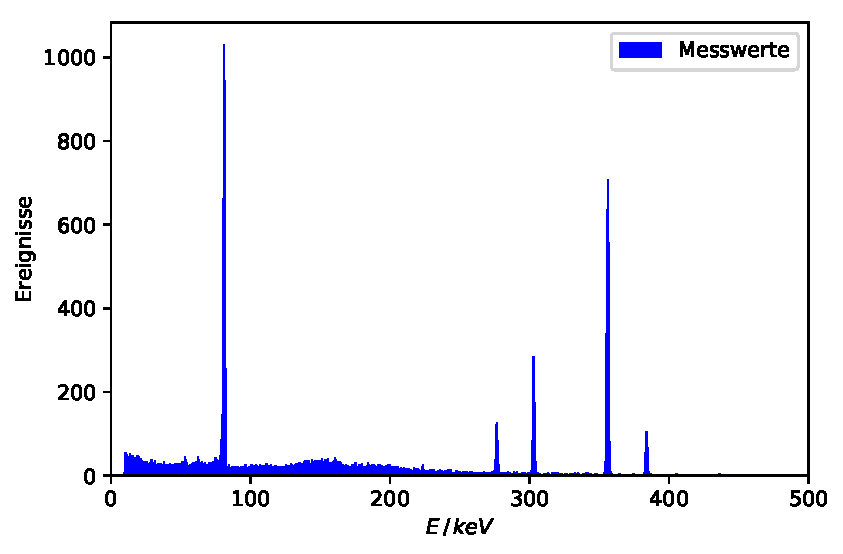
\includegraphics[width=.7\textwidth]{../Plots/Ba_Spektrum.pdf}
  \caption{Spektrum der \ce{^133Ba} Quelle.}
  \label{fig:Ba_Spektrum}
\end{figure}

\subsection{Untersuchung des unbekannten Strahlers}

Zur Bestimmung der unbekannten Strahlenquelle werde die Emissionsenergien der Photopeaks in dem aufgenommenen Spektrum bestimmt.
Mit \cite{Isotopenbestimmung} werden die Emissionsenergien Isotopen zugeordnet.
Dabei fällt auf, dass viele Emissionsenergien zu Isotopen passen, welche Zerfallsprodukte in der Uran-Radium-Reihe sind. Die Emissionsenergien und die dazugehörigen Isotope sind in Tabelle \ref{tab:Uran_Zerfall} aufgetragen.
Die unbekannte Quelle enthält somit wahrscheinlich \ce{^238U}.

Wie schon in Kapitel \ref{sec:Ba} kann aus den Peaks dieser Energien die Aktivität des Urans mit Gleichung \eqref{eqn:Act_Ba} bestimmt werden.
\begin{equation}
  A_\text{\ce{^238U}}(04.11.2019) = \SI{1.4(9)e4}{\becquerel}
\end{equation}

\begin{table}[H]
  \centering
  \caption{Die zur Uran-Radium-Reihe gehörenden Isotope mit ihren im Spektrum gefundenen Emissionsenergien.}
  \label{tab:Uran_Zerfall}
  \begin{tabular}{cc}
    \toprule
    $E_\text{Emission} \, / \, \si{\kilo\electronvolt}$ & Isotop \\
    \midrule
    \num{ 187.0} &  \ce{^226Ra} \\
    \num{ 241.5} &  \ce{^214Pb} \\
    \num{ 295.2} &  \ce{^214Pb} \\
    \num{ 351.9} &  \ce{^214Pb} \\
    \num{ 609.0} &  \ce{^214Bi} \\
    \num{1120.0} &  \ce{^210Bi} \\
    \num{ 768.0} &  \ce{^214Bi} \\
    \num{1237.0} &  \ce{^214Bi} \\
    \num{1377.0} &  \ce{^214Bi} \\
    \bottomrule
  \end{tabular}
\end{table}

\begin{figure}[H]
  \centering
  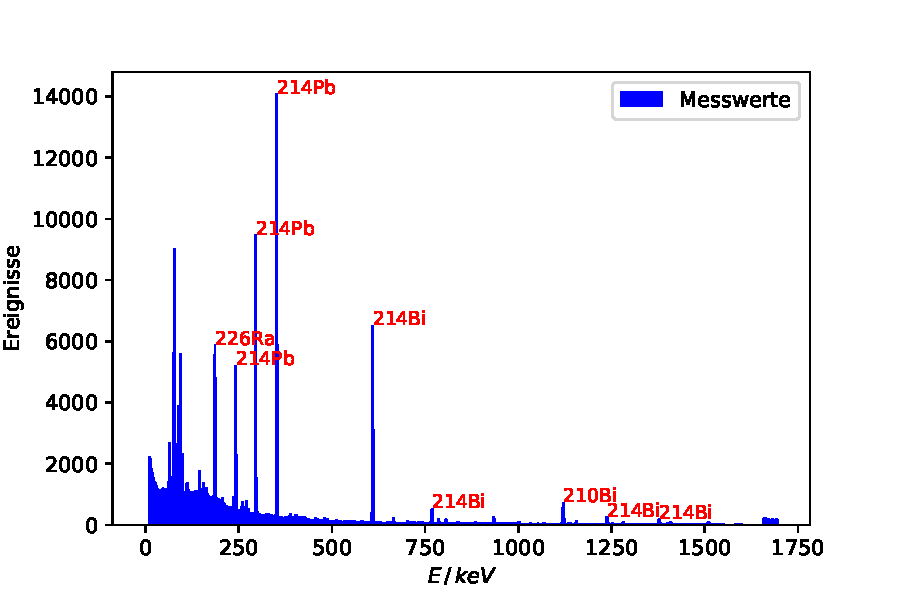
\includegraphics[width=.7\textwidth]{../Plots/U_Spektrum.pdf}
  \caption{Spektrum der \ce{^238Eu} Quelle.}
  \label{fig:U_Spektrum}
\end{figure}
